
\documentclass[a4paper,twoside]{refart}

\usepackage{longtable}
\usepackage{graphicx} 
\usepackage[bitheight=6ex]{bytefield}
\usepackage{gensymb}
\usepackage[stable]{footmisc}
\usepackage{multirow}
\usepackage{hyperref}
\usepackage[toc]{glossaries}

\makeglossaries

\usepackage{hyperref}
\hypersetup{
    colorlinks,
    citecolor=black,
    filecolor=black,
    linkcolor=black,
    urlcolor=blue
}

\usepackage{listings} % Required for inserting code snippets
\usepackage[usenames,dvipsnames]{color} % Required for specifying custom colors and referring to colors by name

\usepackage{pgfgantt}
\usepackage{tikz-timing}

\definecolor{highlight}{RGB}{255,251,204} % Code highlight color

\lstdefinelanguage{sms}
{morekeywords={code,gprs?,setup?,fix?,apn,user,pass,srv,port,vref,err.*,spl,spw,spi,spg,sml,smst,smmt,ping,set,default},
sensitive=false,
morestring=[b]",
}

\lstset{
language=sms, % Detects keywords, comments, strings, functions, etc for the language specified
backgroundcolor=\color{highlight}, % Set the background color for the snippet - useful for highlighting
basicstyle=\footnotesize\ttfamily, % The default font size and style of the code
%basicstyle=\ttfamily, % The default font size and style of the code
breakatwhitespace=false, % If true, only allows line breaks at white space
breaklines=true, % Automatic line breaking (prevents code from protruding outside the box)
captionpos=b, % Sets the caption position: b for bottom; t for top
deletekeywords={}, % If you want to delete any keywords from the current language separate them by commas
%escapeinside={\%}, % This allows you to escape to LaTeX using the character in the bracket
firstnumber=1, % Line numbers begin at line 1
frame=single, % Frame around the code box, value can be: none, leftline, topline, bottomline, lines, single, shadowbox
frameround=tttt, % Rounds the corners of the frame for the top left, top right, bottom left and bottom right positions
keywordstyle=\color{Blue}\bf, % Functions are bold and blue
morekeywords={}, % Add any functions no included by default here separated by commas
numbers=left, % Location of line numbers, can take the values of: none, left, right
numbersep=10pt, % Distance of line numbers from the code box
numberstyle=\tiny\color{Gray}, % Style used for line numbers
rulecolor=\color{black}, % Frame border color
showstringspaces=false, % Don't put marks in string spaces
showtabs=false, % Display tabs in the code as lines
stepnumber=5, % The step distance between line numbers, i.e. how often will lines be numbered
stringstyle=\color{Purple}, % Strings are purple
tabsize=2, % Number of spaces per tab in the code
}

\renewcommand*{\familydefault}{\sfdefault}
%\renewcommand*{\familydefault}{\rmdefault}
%\renewcommand*{\familydefault}{\ttdefault}
%\renewcommand*{\familydefault}{\rmdefault{ppl}}

\newglossaryentry{adc}{%
  name={ADC},
  description={analog to digital converter}
}

\newglossaryentry{cell-id}{%
  name={cell ID},
  description={cell identification code - part of the cell tower id broadcast}
}

\newglossaryentry{cell-lac}{%
  name={cell LAC},
  description={location area code - part of the cell tower id broadcast}
}

\newglossaryentry{cell-mcc}{%
  name={cell MCC},
  description={mobile country code - part of the cell tower id broadcast}
}

\newglossaryentry{cell-mnc}{%
  name={cell MNC},
  description={mobile network code - part of the cell tower id broadcast}
}

\newglossaryentry{cell-rxl}{%
  name={cell RXL},
  description={receive signal strength level - part of the cell tower id broadcast}
}

\newglossaryentry{m2m}{%
  name={M2M},
  description={machine to machine data plan - mobile subscription that covers SMS and data but no voice}
}

\newglossaryentry{pdop}{%
  name={PDOP},
  description={(3D) position dilution of precision - a value that describes the measurement's precision based on satellite geometry scattering as viewed from the ground. the lower the number the better. if it's more than 5 the calculated geographical position is not to be taken into account}
}

\newglossaryentry{f-ram}{%
  name={F-RAM},
  description={Ferroelectric RAM, is a type of non-volatile random-access memory that has far greater write-erase cycle performance than eeprom/flash/SD cards and lower power usage than DRAM, but it has storage capacity limitations that makes it more costly}
}

%\newglossaryentry{}{%
%  name={},
%  description={}
%}


\begin{document}
\title{Gps tracking module with gprs connectivity}
\author{Petre Rodan \url{http://www.simplex.ro}}
\date{created September 2014, revised \today}
\maketitle

\begin{abstract}
This module can be used to track goods wherever gsm signal is present. It is optimized for very low power consumption and has configurable timings which would make it fit to any use scenario.
\end{abstract}


\tableofcontents
\newpage

\section{principles of operation}
Geographic coordinates are obtained by decoding NMEA sentences received from the GPS chipset and then transmitted via the mobile phone network to a web server. The server stores the received information into a database and provides it on demand to the end-user.

Cell tower identifiers are also transmitted in the same packet and this allows approximate localization when the gps signal is obstructed. When the gsm signal is missing data is being stored on the device and it's transmission will resume once connection is re-established.

\section{Quick reference guide}

\subsection{Getting started}

\subsubsection{Requirements}

\marginlabel{Warning} Special care must be taken with the gprs antenna. It has to be connected to the connector marked 'gprs' at all times or otherwise the module could be damaged.

This module works best with two power sources. One 3.7V Li-Polymer/Li-Ion cell (at least 2000mAh recommended) and a 5V input DC that is only used for recharging the cell. Only the second one is optional due to the fact that for very short bursts the gprs modem needs more current than the DC input can handle. This circuitry is USB power friendly. If the module gets installed onto a vehicle, a high efficiency DC-DC converter can be provided to lower the voltage from up to 24V to the 5V needed. Double check the polarity on the connectors before attempting to apply any power to the device. Pin 1 is marked on the silkscreen with a small triangle and that represents the ground (negative) terminal for both the battery and the DC inputs.

The user will also need a mobile phone in order to send commands to the module via SMS and a web browser to visualize the generated data.

\subsubsection{SIM cards and initial setup}

Below is a step-by-step guide for installing a local SIM card into the tracking module. The setup of a 'Vodafone prepay card' is shown as an example.

\begin{itemize}
    \item buy a SIM card. any SIM card will do: prepay-ed, subscription (but do keep in mind that no voice transmission will ever be used on this SIM tho), machine to machine (also known as \gls{m2m}). mini SIM form factor cards are needed.
    \item obtain the associated phone number and enter it into your phone's address-book - don't forget to also add the country prefix so you can contact the tracker while abroad. it's "+4" prefixed to the number in Romania.
    \item place the newly purchased SIM card into an actual phone
    \item if it has no initial credit, fill it with at least 5EUR
    \item make sure no PIN is set on the SIM itself
    \item disable any 'best value plan' the provider might have selected - this SIM will mostly be used to connect to the internet, and it will send a minimal number of SMS messages during the setup process. the only extra options that are needed are the cheapest internet plan available ('100MB internet for 1 Month - 2EUR' for vodafone). also activate data roaming.
    \item disable 'VOX voicemail' by calling \#\#002\#
    \item place the SIMs back into their proper locations: the newly purchased one in the tracker and your old one into the phone.
    \item while inserting the SIM into the tracker write down the last 4 IMEI digits that you see written on the SIM900 IC that is adjacent to the SIM holder.
    \item send a SMS from the phone to the tracker that contains:

\begin{lstlisting}
code 5551
\end{lstlisting}

'5551' will need to be replaced by those digits you wrote down during the previous step

    \item power on the tracker and wait. it only connects to the gsm network every 15 minutes by default and it has a 1 minute interval in which it's actively listening to incoming SMS messages. once the code is received and acknowledged you will get a 'code ok' reply on the phone. from this moment on you can send commands to the tracker.
\end{itemize}

\subsection{gprs setup}

In order for the module to connect to the internet to send out the tracking data it needs a working gprs connection to the mobile service provider. This connection is established only if a set of credentials (\verb"apn", \verb"username" and \verb"password") are used to authenticate the device. You can ask your mobile phone company to provide these. Sometimes one company has customized \verb"apn" and/or \verb"usernmames" for each sim card type, so don't rely on web searches.

Once you get your correct credentials, send them as 3 different SMS commands to the device:

\begin{lstlisting}
apn STRING
\end{lstlisting}
\begin{lstlisting}
user STRING
\end{lstlisting}
\begin{lstlisting}
pass STRING
\end{lstlisting}

\marginlabel{Warning} All strings can be max 20 characters long. If you need more on any of them please contact me.

You can check if all data has been received ok with the following command:

\begin{lstlisting}
gprs?
\end{lstlisting}


\subsection{Web visualization of data}

You can check all the info the tracker sends out by visiting \\ \verb"http://www.simplex.ro/scripts/l1?i=IMEI_NUMBER" .\\
the \verb"IMEI_NUMBER" is a 15 digit number and it's written on the sim900 module.

This project offers the possibility to advanced users to redirect the tracking data to another web server.
Two commands control the location where HTTP POST packets are sent:

\begin{lstlisting}
srv your.server.com
\end{lstlisting}

\begin{lstlisting}
port port_number
\end{lstlisting}

\marginlabel{Warning} All strings can be max 20 characters long. If you need more on any of them please contact me.

The post request will be sent to \verb"http://your.server.com:port_number/u1". u1 has to be a CGI script (or an alias to one) that decodes the binary packets sent. See Section~\ref{sec:post-packets} for details.

\subsection{SMS commands}

\begin{tabular}{ |l|p{8cm}| }
    \hline
        command & 
\begin{lstlisting}
code STRING
\end{lstlisting} \\
        action & pair a phone to the tracker.
STRING has to be the last 4 digits of the SIM900's IMEI \\ \hline
\end{tabular}


\begin{tabular}{ |l|p{8cm}| }
    \hline
        command & 
\begin{lstlisting}
gprs?
\end{lstlisting} \\
        action & show APN, USER, PASSWORD that are currently used in order to authenticate for a gprs session \\ \hline
\end{tabular}


\begin{tabular}{ |l|p{8cm}| }
    \hline
    \multicolumn{2}{|l|}{} \\
    \hline
        command & 
\begin{lstlisting}
setup?
\end{lstlisting} \\
        action & show a hex value containing current switches \\ \hline
\end{tabular}


\begin{tabular}{ |l|p{8cm}| }
    \hline
        command & 
\begin{lstlisting}
fix?
\end{lstlisting} \\
        action & 
try to send back a GPS fix as a SMS reply \\ \hline
\end{tabular}

\begin{tabular}{ |l|p{8cm}| }
    \hline
        command & 
\begin{lstlisting}
ping
\end{lstlisting} \\
        action & 
a HTTP POST is sent with all available data once this command is received \\ \hline
\end{tabular}

\begin{tabular}{ |l|p{8cm}| }
    \hline
        command & 
\begin{lstlisting}
default
\end{lstlisting} \\
        action & 
restores ALL variables to the factory defaults and reboots the device. the user will have to use the \verb"code" command again to pair it's phone\\ \hline
\end{tabular}


\begin{tabular}{ |l|p{8cm}| }
    \hline
        command & 
\begin{lstlisting}
apn STRING
\end{lstlisting} \\
        default & live.vodafone.com \\
        action & 
set the gprs apn value - max 20 char long

in case STRING is missing, an empty apn is used \\ \hline
\end{tabular}


\begin{tabular}{ |l|p{8cm}| }
    \hline
        command & 
\begin{lstlisting}
user STRING
\end{lstlisting} \\
        default & live \\
        action & 
set the gprs user  - max 20 char long

in case STRING is missing, an empty username is used  \\ \hline
\end{tabular}


\begin{tabular}{ |l|p{8cm}| }
    \hline
        command & 
\begin{lstlisting}
pass STRING
\end{lstlisting} \\
        default & vodafone \\
        action & 
set the gprs pass - max 20 char long
in case STRING is missing, an empty password is used  \\ \hline
\end{tabular}


\begin{tabular}{ |l|p{8cm}| }
    \hline
        command & 
\begin{lstlisting}
srv STRING
\end{lstlisting} \\
        default & trk.simplex.ro \\
        action & 
what server to contact in order to send the tracking data \\ \hline
\end{tabular}


\begin{tabular}{ |l|p{8cm}| }
    \hline
        command & 
\begin{lstlisting}
port STRING
\end{lstlisting} \\
        default & 80 \\
        action & 
TCP port used during connection to the server  \\ \hline
\end{tabular}


\begin{tabular}{ |l|p{8cm}| }
    \hline
        command & 
\begin{lstlisting}
vref STRING
\end{lstlisting} \\
        default & 198 \\
        action & 
STRING is a number between 190 and 210 that acts as calibration coefficient to the on board \gls{adc}. only used if the voltage values reported by the module differ from the measured ones \\ \hline
\end{tabular}


\begin{tabular}{ |l|p{8cm}| }
    \hline
        command & 
\begin{lstlisting}
err?
\end{lstlisting} \\
        action & 
shows a hex value in case there were any errors logged in the device. this value gets reset when all power is lost, when an 'err?' command is replied to or after a HTTP POST packet is sent out/stored to \gls{f-ram}. only used for debug  \\ \hline
\end{tabular}

\begin{tabular}{ |l|p{8cm}| }
    \hline
        command & 
\begin{lstlisting}
spt?
\end{lstlisting} \\
        action & 
shows a list of gps related timing values\\ \hline
\end{tabular}

\begin{tabular}{ |l|p{8cm}| }
    \hline
        command & 
\begin{lstlisting}
smt?
\end{lstlisting} \\
        action & 
shows a list of gprs related timing values\\ \hline
\end{tabular}

\begin{tabular}{ |l|p{8cm}| }
    \hline
        commands & 
\begin{lstlisting}
spl STRING
\end{lstlisting}
\begin{lstlisting}
spw STRING
\end{lstlisting}
\begin{lstlisting}
spi STRING
\end{lstlisting}
\begin{lstlisting}
spg STRING
\end{lstlisting}
\begin{lstlisting}
sml STRING
\end{lstlisting}
\begin{lstlisting}
smst STRING
\end{lstlisting}
\begin{lstlisting}
smmt STRING
\end{lstlisting} \\
        action &
timing variables. see section \ref{sub:timing} for details.
\\ \hline
\end{tabular}


\section{developer guide}
\subsection{software}

All the documentation, sources and hardware schematics are provided as Open Source in order to encourage further improvements by the community. The TI spy-bi-wire protocol can be used to re-flash the enclosed microcontroller.

Firmware is written in C and it's created to be fully non-blocking and interrupt driven. The server-side scripts are in perl and bash.

Any web server can be used to receive the binary data sent from the tracker. The unpack() function present in perl, python, php will reconstruct the information and make it ready to be inserted into a database. Special care has to be taken so that the web server's reply header is as short as possible. If it's too long the module will not parse it properly and the data flow will be disrupted. In case nginx is used using the following settings are highly recommended:

\begin{lstlisting}
more_clear_headers 'Server';
more_clear_headers 'Date';
more_clear_headers 'Content-Type';
more_clear_headers 'Transfer-Encoding';
more_clear_headers 'Connection';
\end{lstlisting}

Provided scripts have the following run time dependencies (some are optional):

\begin{itemize}
    \item perl at least ver 5.8.2
    \item sqlite at least ver 3.0.0
    \item bash
    \item nginx
    \item fcgi
\end{itemize}

\subsubsection{tweaking the firmware}

the original source code is kept in a git repository at github.com.
one can grab a copy by running

\begin{lstlisting}
git clone http://github.com/rodan/tracy
\end{lstlisting} 

or by downloading a snapshot archive

\begin{lstlisting}
wget https://github.com/rodan/tracy/archive/master.zip
\end{lstlisting} 

compiling is as easy as
\begin{lstlisting}
cd firmware
make clean
make
\end{lstlisting} 

the following packages are used to compile and manage the firmware:

\begin{itemize}
    \item msp430-gcc (ver 4.6.3\_p20120406 has been used)
    \item msp430-binutils (2.22\_p20120911)
    \item msp430-libc (20120716)
    \item msp430mcu (20120716)
    \item mspdebug (0.22)
\end{itemize}

burning the firmware can be achieved with any MSP430 programmer that supports SPY-Bi-Wire. 

\marginlabel{Warning} specialized programmers can detect the 2.8V rail the microcontroller uses and will not send signals with a higher voltage. anything higher than 3V is just asking for trouble. 

mspdebug can be used to program the firmware:

\begin{lstlisting}
mspdebug rf2500 "prog proj.elf"
\end{lstlisting}

\subsubsection{HTTP POST packets}
\label{sec:post-packets}

Tracking information is sent to the server by TCP packets via the HTTP POST method. A web server is thus needed to receive the data and feed it to the parsing script (see \verb"server/scripts/u1" in the repository).

In order to have a good bandwidth usage the data is sent in a binary format and the \gls{f-ram} chip that is being used allows the data to be buffered and sent out at set intervals. Most scripting languages have an unpack() function that can correctly decode these packets. A sample perl script is provided in the repository (see \verb"server/scripts/l1").

Each positional measurement will be placed in a subsegment. At least one of these subsegments will constitute one segment that is sent out together with a HTTP header to create an HTTP POST request (see Figure~\ref{fig:packet-format}).

\begin{figure}[htbp]
  \centering
  \begin{bytefield}{32}
    \bitheader{0,0} \\
    \begin{rightwordgroup}{HTTP \\ POST \\ method \\ header}
        \bitbox{32}{POST /u1 HTTP/1.0} \\
        \bitbox{32}{Host: trk.simplex.ro} \\
        \bitbox{32}{Content-Type: application/binary} \\
        \bitbox{32}{Content-Length: 00000}
    \end{rightwordgroup} \\

    \begin{rightwordgroup}{one\\ segment}
    \wordbox[lrt]{1}{
      \parbox{0.6\width}{\centering at least one subsegment}} \\
    \skippedwords \\
    \wordbox[lrb]{1}{} 
  \end{rightwordgroup}
  \end{bytefield}
  \caption{packet format}
  \label{fig:packet-format}
\end{figure}

\begin{figure}[htbp]
  \centering
  \begin{bytefield}{32}
    \bitheader{0,7-8,15-16,23-24,31} \\
    \begin{rightwordgroup}{subsegment \\ header}
        \bitbox{16}{version} &&
        \bitbox[tlr]{16}{} \\
        \wordbox[lr]{1}{\parbox{0.6\width}{\centering 15 byte IMEI}} \\
        \skippedwords \\
        \wordbox[lrb]{1}{} \\ 
        \bitbox{16}{settings} &&
        \bitbox{16}{$V_{BAT}$} \\
        \bitbox{16}{$V_{RAW}$} &&
        \bitbox{16}{errors} \\
        \bitbox{16}{message id} &&
        \bitbox{8}{payload descriptor} &&
        \bitbox[tlr]{8}{} \\
        \bitbox[rl]{32}{timestamp} \\
        \bitbox[rlb]{8}{} &&
        \bitbox[tl]{24}{}
    \end{rightwordgroup} \\
    \begin{rightwordgroup}{payload}
    \\
    \bitbox[lrb]{32}{\dots gps and/or gprs payload}
    \end{rightwordgroup}
  \end{bytefield}
  \caption{subsegment format}
  \label{fig:subsegment-format}
\end{figure}

\begin{figure}[htbp]
  \centering
  \begin{bytefield}{32}
    \bitheader{0,7-8,15-16,23-24,31} \\
    \begin{rightwordgroup}{gps \\ data}
        \bitbox{32}{latitude (float)} \\
        \bitbox{32}{longitude (float)} \\
        \bitbox{16}{\gls{pdop}} &&
        \bitbox{16}{speed} \\
        \bitbox{16}{heading} &&
        \bitbox{16}{system time} \\
        \bitbox{16}{system time} &&
        \bitbox[btl]{16}{geofence distance} \\
        \bitbox[btr]{16}{geofence distance} &&
        \bitbox{16}{geofence bearing}
    \end{rightwordgroup}
  \end{bytefield}
  \caption{gps payload}
  \label{fig:gps_payload}
\end{figure}

\begin{figure}[htbp]
  \centering
  \begin{bytefield}{32}
    \bitheader{0,7-8,15-16,23-24,31} \\
    \begin{rightwordgroup}{gprs \\ data}
        \bitbox{16}{\gls{cell-rxl}} &&
        \bitbox{16}{\gls{cell-mcc}} \\
        \bitbox{16}{\gls{cell-mnc}} &&
        \bitbox{16}{\gls{cell-id}} \\
        \bitbox{16}{\gls{cell-lac}}
    \end{rightwordgroup}
  \end{bytefield}
  \caption{gprs payload}
  \label{fig:gprs_payload}
\end{figure}

Each subsegment (shown in Figure~\ref{fig:subsegment-format}) has a header containing the timestamp at the time of the fix, modem IMEI, system voltages, previous errors detected, basic device configuration, an auto increment id and a byte that describes the type of the positional data. This can either be a GPS fix (Figure~\ref{fig:gps_payload}) and/or one up to four tower identification strings (Figure~\ref{fig:gprs_payload}).

The tower identification strings are post-processed on the web server and a \emph{very} approximate geographic position is obtained.

These subsegments are simply concatenated together to constitute the final segment being sent. The size of one such segment varies but SIM900's internal buffering limits it up to 1000bytes. During one GPRS session one up to \verb"MAX_SEG" are sent out at a time. If GPRS connections cannot be established for a long interval and \verb"MAX_SEG" is reached then the oldest segment is freed in order to make place for new data.

\newpage
\subsubsection{Timings and intervals}
\label{sub:timing}

This tracking module allows fine-grained timing customization. It can either preserve battery life for more than a month when sparse measurements are being made or it can record positional data every 10 seconds if needed. Either behavior can be set by the user via SMS commands, without the need to change the firmware.

A 'reset to factory settings' function is also provided in case the user needs to return to known-good timing values.

Default values for the gps intervals are depicted in Table~\ref{gps_diag}. The yellow time intervals are configurable: the entire loop takes 180 seconds - from which in the first 135 the gps module is powered off, a 45 sec warmup brings the device to life and it should be enough to ensure a good fix at the end of that interval. During the invalidation period the module will choose the fix with the best \gls{pdop} value and that will get stored into \gls{f-ram}.

\begin{table}[ht]
\begin{ganttchart}[
vgrid,
bar/.append style={fill=yellow, rounded corners=3pt},
bar left shift=.15,
bar right shift=-.15,
bar top shift=.4,
bar height=.2,
group left shift=0,
group right shift=0,
group peaks tip position=0,
group peaks height=.4,
milestone/.append style={fill=orange, rounded corners=3pt}
]{0}{18}
\ganttbar{loop}{0}{18} \\
\ganttbar{warmup}{13}{18} \\
\ganttbar{invalidate}{16}{18} \\
\ganttmilestone{store fix}{18} \\
\ganttbar[bar/.append style={fill=gray}]{gps off/on}{0}{12}
\ganttbar[bar/.append style={fill=red}]{}{13}{18}
\end{ganttchart}
\caption{\em default time intervals for the gps subsystem}
\label{gps_diag}
\end{table}

If much more frequent gps data needs to be acquired, ie\\
\verb"loop interval" $\leq$ \verb"warmup interval" + \verb"30s" \\
then the gps will never be powered off. See Table~\ref{gps_diag_10s} for an example where all gps intervals are set to 10 seconds.

\begin{table}[ht]
\begin{ganttchart}[
vgrid,
bar/.append style={fill=yellow, rounded corners=3pt},
bar left shift=.15,
bar right shift=-.15,
bar top shift=.4,
bar height=.2,
group left shift=0,
group right shift=0,
group peaks tip position=0,
group peaks height=.4,
milestone/.append style={fill=orange, rounded corners=3pt}
]{0}{18}
\ganttbar{loop}{0}{18} \\
\ganttbar{warmup}{0}{18} \\
\ganttbar{invalidate}{0}{18} \\
\ganttmilestone{store fix}{18} \\
\ganttbar[bar/.append style={fill=gray}]{gps off/on}{0}{0}
\ganttbar[bar/.append style={fill=red}]{}{0}{18}
\end{ganttchart}
\caption{\em 10s loop for the gps subsystem}
\label{gps_diag_10s}
\end{table}

As a rule of thumb try to have at least 45 seconds as the warmup interval in case the gps gets powered off.
And given the fact that the gps is set to send data every two seconds to the microcontroller make sure the invalidation interval is at least 6-8 seconds.

Unlike the gps, the gsm modem needs to be kept off most of the time since it is by far the most power hungry subsystem on this module.
Also a little known fact is that internet data plans have small hidden costs that can add up in time. Sometimes there is a minimum data unit (between 1-10kbytes) that gets counted for every established gprs connection, also while in roaming each gprs initialization has a cost associated with it.
So depending on your gsm provider and use case, you want to get the best trade-off using the configurable variables described in this section.

The modem gets woken up by one of these two triggers:

\begin{itemize}
    \item a periodic check for any new SMS command to be acted upon. this wake-up has no costs associated with it if no SMS reply is to be sent back to the user \\ trigger controlled by \verb"gprs loop interval"
    \item upload of data stored in \gls{f-ram} via gprs. SMS commands are also accepted at this point. this trigger can happen either because enough data has piled up in the memory, one of the \verb"gprs tx interval"s has been reached, the \verb"ping" command was received or the module just started to move after being stationary. \\ trigger controlled by \verb"gprs static tx interval" when the module is not moving or \verb"gprs moving tx interval" otherwise.
\end{itemize}

Whatever is the reason for the modem startup, the neighboring tower cell IDs are stored as a secondary (but less precise) positioning method. 

The module behavior when using the default gprs interval settings is shown in a simplified form in Table~\ref{gsm_diag}. Every 900 seconds the \verb"gprs loop interval" wakes up the modem for a 2 minute period in which possible SMSs are parsed and tower cell IDs are captured.

A movement that was detected triggers an upload of data and makes the next upload happen after 600sec (\verb"gprs moving tx interval"). The next transfer will happen after 3600sec (\verb"gprs static tx interval") since the module is not moving.

\begin{table}[ht]
\scalebox{0.48}{
\begin{tikztimingtable}
 loop trigger & 1H 9L 1H 9L 1H 9L 1H 9L 1H 9L 1H 9L 1H 9L 1H 9L 1H 4L\\
 movement & 2L 3H 80L \\
 tx trigger & 2L 1H 6L 1H 36L 1H 36L 1H 1L \\
\extracode
    \tablerules
\end{tikztimingtable}
}
\caption{\em default module behavior}
\label{gsm_diag}
\end{table}


\subsubsection{list of timing variables}

\label{sms:spl}
\begin{tabular}{ |l|c|c|c|c| }
    \hline
    \multicolumn{1}{|c|}{\multirow{2}{*}{\textbf{gps loop interval}}} & \multicolumn{3}{|c|}{value} & \multicolumn{1}{|c|}{\multirow{2}{*}{unit}} \\ \cline{2-4}
    \multicolumn{1}{|c|}{} & min & default & max & \\ \hline
    value & 10 & 180 & 65535 & seconds \\ \hline
    sms command to set & \multicolumn{4}{|l|}{\textbf{spl} $value$} \\ \hline
    sms command to view & \multicolumn{4}{|l|}{\textbf{spt?}} \\ \hline
    description & \multicolumn{4}{|p{7cm}|}{sets the interval between two gps measurement sessions} \\ \hline
\end{tabular}

\label{sms:spw}
\begin{tabular}{ |l|c|c|c|c| }
    \hline
    \multicolumn{1}{|c|}{\multirow{2}{*}{\textbf{gps warmup interval}}} & \multicolumn{3}{|c|}{value} & \multicolumn{1}{|c|}{\multirow{2}{*}{unit}} \\ \cline{2-4}
    \multicolumn{1}{|c|}{} & min & default & max & \\ \hline
    value & 0 & 45 & 65535 & seconds \\ \hline
    sms command to set & \multicolumn{4}{|l|}{\textbf{spw} $value$} \\ \hline
    sms command to view & \multicolumn{4}{|l|}{\textbf{spt?}} \\ \hline
    description & \multicolumn{4}{|p{7cm}|}{time interval between gps powerup and the actual measurement} \\ \hline
\end{tabular}

\label{sms:spi}
\begin{tabular}{ |l|c|c|c|c| }
    \hline
    \multicolumn{1}{|c|}{\multirow{2}{*}{\textbf{gps invalidate interval}}} & \multicolumn{3}{|c|}{value} & \multicolumn{1}{|c|}{\multirow{2}{*}{unit}} \\ \cline{2-4}
    \multicolumn{1}{|c|}{} & min & default & max & \\ \hline
    value & 0 & 20 & 65535 & seconds \\ \hline
    sms command to set & \multicolumn{4}{|l|}{\textbf{spi} $value$} \\ \hline
    sms command to view & \multicolumn{4}{|l|}{\textbf{spt?}} \\ \hline
    description & \multicolumn{4}{|p{6.8cm}|}{time interval at the end of the measurement session during which the gps fix with the best \gls{pdop} is searched for} \\ \hline
\end{tabular}

\verb"spi" must be a smaller value then \verb"spl".

\label{sms:spg}
\begin{tabular}{ |l|c|c|c|c| }
    \hline
    \multicolumn{1}{|c|}{\multirow{2}{*}{\textbf{gps geofence trigger}}} & \multicolumn{3}{|c|}{value} & \multicolumn{1}{|c|}{\multirow{2}{*}{unit}} \\ \cline{2-4}
    \multicolumn{1}{|c|}{} & min & default & max & \\ \hline
    value & 0 & 300 & 65535 & meters \\ \hline
    sms command to set & \multicolumn{4}{|l|}{\textbf{spg} $value$} \\ \hline
    sms command to view & \multicolumn{4}{|l|}{\textbf{spt?}} \\ \hline
    description & \multicolumn{4}{|p{7cm}|}{minimal distance between two consecutive fixes at which the device is considered non-stationary} \\ \hline
\end{tabular}

Heavy cloud coverage or large adjacent buildings can obscure or create multipath errors in the gps signal detection. It is thus advisable to not set the \textbf{spg} variable too low in order to minimize false-positives.

\label{sms:sml}
\begin{tabular}{ |l|c|c|c|c| }
    \hline
    \multicolumn{1}{|c|}{\multirow{2}{*}{\textbf{gprs loop interval}}} & \multicolumn{3}{|c|}{value} & \multicolumn{1}{|c|}{\multirow{2}{*}{unit}} \\ \cline{2-4}
    \multicolumn{1}{|c|}{} & min & default & max & \\ \hline
    value & 180 & 900 & 65535 & seconds \\ \hline
    sms command to set & \multicolumn{4}{|l|}{\textbf{sml} $value$} \\ \hline
    sms command to view & \multicolumn{4}{|l|}{\textbf{smt?}} \\ \hline
    description & \multicolumn{4}{|p{7cm}|}{time interval between two gsm connection attempts (these are used to get tower id data and to receive and parse sms commands)} \\ \hline
\end{tabular}

each application needs a different trade-off between sms responsiveness and low power consumption.

\label{sms:smst}
\begin{tabular}{ |l|c|c|c|c| }
    \hline
    \multicolumn{1}{|c|}{\multirow{2}{*}{\textbf{gprs static tx interval}}} & \multicolumn{3}{|c|}{value} & \multicolumn{1}{|c|}{\multirow{2}{*}{unit}} \\ \cline{2-4}
    \multicolumn{1}{|c|}{} & min & default & max & \\ \hline
    value & 180 & 3600 & 65535 & seconds \\ \hline
    sms command to set & \multicolumn{4}{|l|}{\textbf{smst} $value$} \\ \hline
    sms command to view & \multicolumn{4}{|l|}{\textbf{smt?}} \\ \hline
    description & \multicolumn{4}{|p{7cm}|}{time interval between two HTTP POSTs when the device is stationary (see \textbf{spg} \ref{sms:spg})} \\ \hline
\end{tabular}

\label{sms:smmt}
\begin{tabular}{ |l|c|c|c|c| }
    \hline
    \multicolumn{1}{|c|}{\multirow{2}{*}{\textbf{gprs moving tx interval}}} & \multicolumn{3}{|c|}{value} & \multicolumn{1}{|c|}{\multirow{2}{*}{unit}} \\ \cline{2-4}
    \multicolumn{1}{|c|}{} & min & default & max & \\ \hline
    value & 180 & 600 & 65535 & seconds \\ \hline
    sms command to set & \multicolumn{4}{|l|}{\textbf{smmt} $value$} \\ \hline
    sms command to view & \multicolumn{4}{|l|}{\textbf{smt?}} \\ \hline
    description & \multicolumn{4}{|p{7cm}|}{time interval between two HTTP POSTs when the device is moving (see \textbf{spg} \ref{sms:spg})} \\ \hline
\end{tabular}

all the timings in this section are used for scheduling the respective actions. the final timestamps received in the web reports will not follow exactly the values entered. this happens because the device tries to get the best fix possible in the \textbf{spi} interval based on \gls{pdop} measurements and also because most actions performed are dependent on both outside factors (how quickly a good fix is received from the gps, mobile service availability, how many sms actions need to be executed) as well as local interactions (the gprs modem can only perform one task at any given time).

\newpage
\subsection{hardware}

\marginlabel{MSP430F5510 mixed signal microcontroller}
    \begin{itemize}
        \item 16bit RISC architecture with 32KB flash and 4KB of SRAM
        \item low supply voltage - 2.8V used in this implementation
        \item ultra-low power consumption
        \item 10bit \gls{adc} - both the battery voltage and input voltage levels are kept in check
        \item 4 16bit timers with interrupt generation - used to synchronize all processes
        \item real-time clock - keeps calendar data and the clock when gps signal is missing
        \item port mapping controller - allows digital functions to be switched between different ports
        \item watchdog, brown out reset - ensures the system runs in stable parameters
    \end{itemize}

\marginlabel{SIM900 quad-band GSM/GPRS engine}
    \begin{itemize}
        \item GSM 850MHz, EGSM 900MHz, DCS 1800MHz, PCS 1900MHz frequencies are supported
        \item a dedicated user-provided micro SIM is needed to connect to the mobile phone network of choice. \gls{m2m} SIMs also work since voice is never used in this application.
    \end{itemize}

\marginlabel{MT3339 MediaTek GPS chipset}
    \begin{itemize}
        \item tiny gps module that can track 22 satellites at any given moment
        \item even if the module is mostly shut down to conserve power, the backup voltage is always provided thus ensuring a fast time-to-fix when started up
        \item automatic antenna switching detects external antennas
    \end{itemize}
\marginlabel{BQ24072 power path management IC}
    \begin{itemize}
        \item allows charging of the Li-Ion/LiPo cell from a USB friendly 5V source
        \item maximum charging current is limited to 300mA
    \end{itemize}
\marginlabel{FM24V10 IC}
    \begin{itemize}
        \item additional 1Mbit \gls{f-ram} for data buffering and storage
    \end{itemize}
\marginlabel{accu}
    \begin{itemize}
        \item 1 cell LiPo battery for standalone operation
    \end{itemize}

\subsubsection{absolute maximum ratings}

\begin{tabular}{ |c|c|l|c|c|c| }
    \hline
    \multicolumn{3}{|c|}{} & \multicolumn{2}{|c|}{value} & unit \\ \cline{4-6}
    \multicolumn{3}{|c|}{} & min & max & \\ \hline
    \multicolumn{1}{|c|}{\multirow{2}{*}{$V_{I}$}} & \multicolumn{1}{|c|}{\multirow{2}{*}{input voltage}} &    IN (with respect to VSS) & -0.3    & 28  & V \\ \cline{3-6}
                &                       &  VBAT (with respect to VSS)   & -0.3  & 5   & V \\ \hline
    $V_{IO}$ & \multicolumn{2}{|l|}{IO voltage thru the debug connector}                      & -0.3  & 3.1 & V \\ \hline
    $T_{stg}$   & \multicolumn{2}{|l|}{storage temperature}             & -65   & 150 & \degree C \\  \hline
    $T_{op}$   & \multicolumn{2}{|l|}{operating temperature}          & 0     & 125 & \degree C \\  \hline
\end{tabular}

Stresses above those listed in absolute maximum ratings may cause permanent damage to the device. This is a stress rating only, functional operation of the device at these or any other conditions above those indicated in the operational section of this specification is not implied. Exposure to absolute maximum rating conditions for extended periods may affect device reliability.

\subsubsection{electrical characteristics}

\begin{tabular}{ |c|l|c|c|c|c| }
    \hline
    \multicolumn{2}{|c|}{} & \multicolumn{3}{|c|}{value} & unit \\ \cline{3-6}
    \multicolumn{2}{|c|}{} & min & typ & max & \\ \hline
    $V_{I}$ & input voltage range                      & 4.35  & 5     & 6.4  & V \\ \hline
    $I_{I}$ & input current                            & X     & X     & 1.5  & A \\ \hline
    $V_{BAT}$ & battery voltage range                  & 3.5   &       & 4.1  & V \\ \hline
    $I_{BAT}$ & battery current while discharging      & X     & X     & 2000 & mA \\ \hline
    $I_{CHG}$ & battery charging current \footnotemark &       & 0.3   &   & A \\ \hline
    $V_{IO}$ & IO voltage thru the debug connector     & 0     &       & 2.8  & V \\ \hline
\end{tabular}

\footnotetext{The charging current is configurable by changing the value of R11. See the module schematic and the bq24072 datasheet for details}

\section{connectors}
for all pin connectors, pin 1 is marked by a small triangle in the silkscreen

%\marginlabel{battery thermistor}
\begin{tabular}{ |l|p{8cm}| }
    \hline
    \multicolumn{2}{|l|}{battery thermistor} \\
    \hline
        connector & Molex 053048-0210 \\
        footprint & \begin{center} 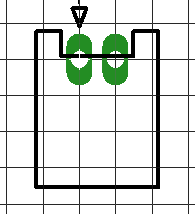
\includegraphics[height=50pt]{img/con2} \end{center} \\ \hline
        silkscreen & \verb"10KOhm ts" \\ \hline
        use & some battery packs provide this component as a charge ending protection. by default this connector is unpopulated and if it's use is required the 10K resistor located on the other side of the PCB needs to be removed \\
    \hline
    \multicolumn{2}{|l|}{pin assignments} \\
    \hline
        1   &   10K NTC thermistor \\
        2   &   10K NTC thermistor (also GND)\\
    \hline
\end{tabular}

\begin{tabular}{ |l|p{8cm}| }
    \hline
    \multicolumn{2}{|l|}{LiPo/Li-Ion 1 cell battery} \\
    \hline
        connector & Molex 053048-0210 \\
        footprint & \begin{center} 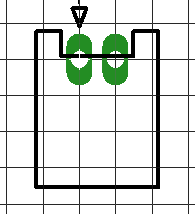
\includegraphics[height=50pt]{img/con2} \end{center} \\ \hline
        silkscreen & \verb"3.7V bat"  \\ \hline
        use & 1 cell (3.7V) rechargeable Li-Ion or Li polymer battery \\
    \hline
    \multicolumn{2}{|l|}{pin assignments} \\
    \hline
        1   &   GND \\
        2   &   +3.7V \\
    \hline
\end{tabular}

\begin{tabular}{ |l|p{8cm}| }
    \hline
    \multicolumn{2}{|l|}{5V DC input} \\
    \hline
        connector & Molex 053048-0210 \\
        footprint & \begin{center} 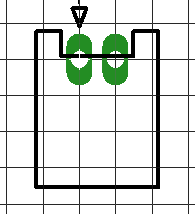
\includegraphics[height=50pt]{img/con2} \end{center} \\ \hline
        silkscreen & \verb"5V" \\ \hline
        use & 5V DC either from a USB connection or a DCDC converter. used only to charge the included battery with a current up to 300mA \\
    \hline
    \multicolumn{2}{|l|}{pin assignments} \\
    \hline
        1   &   GND \\
        2   &   +5V \\
    \hline
\end{tabular}

\begin{tabular}{ |l|p{8cm}| }
    \hline
    \multicolumn{2}{|l|}{programming/debug connector} \\
    \hline
        connector & Molex 053048-0610 \\
        footprint & \begin{center} 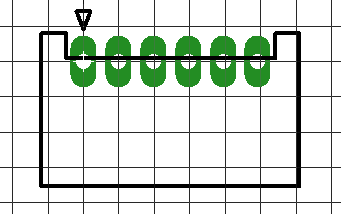
\includegraphics[height=50pt]{img/con6} \end{center} \\ \hline
        silkscreen & \verb"debug" \\ \hline
        use & pins 3-6 are used for TI's spy-bi-wire protocol in order to program or to debug the microcontroller. pins 1 and 2 can have a custom assignation \\
    \hline
    \multicolumn{2}{|l|}{pin assignments} \\
    \hline
        1   &   P4.1 - context dependent microcontroller port \\
        2   &   P4.0 - context dependent microcontroller port \\
        3   &   2.8V - VCC OUT \\
        4   &   TEST \\
        5   &   RST \\
        6   &   GND \\
    \hline
\end{tabular}

\begin{tabular}{ |l|p{8cm}| }
    \hline
    \multicolumn{2}{|l|}{gsm antenna} \\
    \hline
        connector & UFL \\
         & \begin{center} 
\includegraphics[height=40pt]{img/ufl} \end{center} \\ \hline
        silkscreen & \verb"gsm" \\ \hline
        use & it is mandatory to connect the enclosed antenna via this connector \\
    \hline
    \multicolumn{2}{|l|}{pin assignments} \\
    \hline
        shroud   &   GND \\
        center   &   signal \\
    \hline
\end{tabular}

\begin{tabular}{ |l|p{8cm}| }
    \hline
    \multicolumn{2}{|l|}{gps antenna} \\
    \hline
        connector & UFL \\
         & \begin{center} 
\includegraphics[height=40pt]{img/ufl} \end{center} \\ \hline
        silkscreen & \verb"gps" \\ \hline
        use & the gps module provides a small patch antenna but one could improve signal reception by using an external one connected here\\
    \hline
    \multicolumn{2}{|l|}{pin assignments} \\
    \hline
        shroud   &   GND \\
        center   &   signal \\
    \hline
\end{tabular}

\newpage


%\glsaddall
\printglossaries
%\printglossary[type=acronymdesc,style=altlist]

%\printnoidxglossary[type=main,sort=word]
%\printnoidxglossary[type=symbols,sort=use]

%\renewcommand*{\glsnamefont}[1]{\textmd{#1}}

%\printnoidxglossary[type=index,style=mcolindexgroup,sort=word]


\end{document}
